% QEDRank: evaluation methodology (draft, 2026-10-16)
% Companion of the Claude Doc "QEDRank Evaluation Methodology".
% Build: pdflatex methodology.tex  (twice, for the table of contents and references)
\documentclass[11pt,a4paper]{article}
\usepackage[utf8]{inputenc}
\usepackage[T1]{fontenc}
\usepackage{lmodern}
\usepackage[margin=24mm]{geometry}
\usepackage{microtype}
\usepackage{booktabs}
\usepackage{array}
\usepackage{longtable}
\usepackage{amsmath}
\usepackage{amssymb}
\usepackage{enumitem}
\usepackage{xcolor}
\usepackage{graphicx}
\usepackage{tikz}
\usetikzlibrary{arrows.meta,positioning,calc}
\usepackage[hidelinks]{hyperref}

\newcolumntype{L}[1]{>{\raggedright\arraybackslash}p{#1}}
\setlength{\parskip}{4pt plus 1pt}
\setlength{\parindent}{0pt}
\setlength{\tabcolsep}{4pt}
\setlist{nosep}
% Monospace identifiers, paths and hosts may break after - / . and _ (the tt font has
% hyphenation switched off, and names such as /raid/mitarbeiter/<user> have no hyphen).
\ExplSyntaxOn
\NewDocumentCommand{\code}{m}
  {
    \group_begin:
    \ttfamily \hyphenchar \font = 45 \scan_stop:
    \tl_set:Nn \l_tmpa_tl {#1}
    \tl_replace_all:Nnn \l_tmpa_tl {-} {-{}} % keep -- as two hyphens (command-line flags)
    \tl_replace_all:Nnn \l_tmpa_tl {/} {/\allowbreak}
    \tl_replace_all:Nnn \l_tmpa_tl {.} {.\allowbreak}
    \tl_replace_all:Nnn \l_tmpa_tl {\_} {\textunderscore\allowbreak}
    \tl_use:N \l_tmpa_tl
    \group_end:
  }
\ExplSyntaxOff
\setlength{\emergencystretch}{3em} % a long identifier may stretch a line rather than overflow
\newcommand{\pending}{\ensuremath{\square}}

\title{QEDRank: Evaluation Methodology for Lean~4 Proof Benchmarks on ProofBench\\[4pt]
  \large Measuring instruments, validity controls and the state of the runs}
% Replace with the author list and affiliations before circulation.
\author{Author names and affiliations}
\date{16 October 2026 (draft)}

\begin{document}
\maketitle

\begin{abstract}
QEDRank is a single-call evaluator for Lean~4 theorem-proving benchmarks, built around the private ProofBench corpus (111 problems at the commit used for the paper runs). It measures two tasks: \emph{prove} (fill the \code{sorry} of a given formal statement) and \emph{formalize} (write the statement from the paper, then a proof, with a mapping and confidence report). Every answer is compiled in the benchmark's pinned Lean/Mathlib project, checked for \code{sorry} and non-standard axioms, and classified into a fixed verdict set; provider failures (timeouts, rate limits, exhausted quota) are kept apart from model outcomes so they never inflate or deflate a score. Reported statistics are pass@1 with a paper-cluster bootstrap interval in the summary and a Clopper--Pearson interval in the LaTeX tables, the unbiased pass@$k$ estimator of Chen et al.\ for repeated attempts, and McNemar tests with Holm correction for model comparisons.

As of 16 October 2026 no run yet yields reportable model performance. The 11 October pilot (Qwen3-30B-A3B via GWDG, Kimi~K3 via Moonshot) was graded in the wrong Lean project and had a grader import bug; after re-grading, Qwen produced 8 compiling answers out of 109 and 0 verified proofs, and Kimi returned almost nothing because of account limits. The 12 October formalize run inherited the same project problem (65 of 84 reference statements unavailable). Harness fixes for both problems, pass@$k$ support and provider-halt logic are implemented but uncommitted; the pass@8 runs (Kimi~K3, Qwen3) and the self-hosted Qwen3 runs are prepared but not started.

Alongside QEDRank, the paper describes the complementary agentic harness of the ProofBench team (Inspect~AI ReAct agent, up to 10 sessions with handoff notes, two-layer grading with \code{check\_proof.py} and Lean FRO's Comparator), which was set up and verified on a Windows PC with Docker, and the three serving routes tried for an open-weight model: GWDG Chat~AI (200 requests per hour), a vLLM server on the TU Freiberg HPC, and llama.cpp on a DGX-2 with V100 GPUs.
\end{abstract}

\tableofcontents

% ------------------------------------------------------------------
\section{Introduction and scope}

The question is whether current language models can prove, or formalize and prove, research-level mathematics in Lean~4 when the only judge is the Lean kernel. ProofBench supplies the problems: statements taken from recent papers, formalized against Mathlib, kept private so that answers cannot be looked up. This paper describes the measuring instruments, not results.

Two instruments are used, on purpose, because they answer different questions (Table~\ref{tab:instruments}). QEDRank is the baseline and the statistics layer; the agent harness is the shared protocol of the ProofBench team. Both run the same problems from the same private statement repository, so a problem solved by the agent but not in one pass is attributable to tool use rather than to a different corpus.

\begin{table}[htbp]
\centering\small
\caption{The two instruments.}
\label{tab:instruments}
\begin{tabular}{L{26mm}L{58mm}L{66mm}}
\toprule
& QEDRank & ProofBench agent harness (\code{proofbench-eval-apptainer}) \\
\midrule
Protocol & one request per problem and attempt, no tools & ReAct agent with bash, Python, a Lean language server; up to 10 sessions chained by handoff notes \\
Question answered & what the model knows and can write down in one pass & what the model can achieve when it may compile, inspect errors and retry \\
Tasks & prove; formalize (statement + proof + mapping + confidences) & prove \\
Grading & compile in the pinned project, \code{sorry} and axiom check, statement-unchanged check; fidelity check of generated statements & layer~1 \code{check\_proof.py}; layer~2 Comparator (kernel replay in a Landlock sandbox) \\
Statistics & pass@1 with intervals; unbiased pass@$k$; paper-cluster bootstrap; cost & accuracy $\pm$ standard error per run; per-problem \code{results.csv} \\
Author & this project & Utku Okur, ProofBench team \\
\bottomrule
\end{tabular}
\end{table}

What this paper claims: the procedure is defined, implemented, tested on fixtures and live smoke tests, and its failure modes so far are known and recorded. What it does not claim: any score for any model. Section~\ref{sec:runs} lists every run to date and why none is reportable yet.

% ------------------------------------------------------------------
\section{Benchmark corpus}

All prove runs use the private repository \code{proof-bench/proofbench-statements} pinned to one commit; every run folder records that commit, so the problem set of a run is reproducible to the byte. Four snapshots have been used or compared (Table~\ref{tab:corpus}).

\begin{table}[htbp]
\centering\small
\caption{Corpus snapshots.}
\label{tab:corpus}
\begin{tabular}{L{32mm}L{14mm}L{18mm}L{48mm}L{34mm}}
\toprule
Repository and ref & Commit & Date & Problems & Used for \\
\midrule
\code{proofbench-statements} & \code{466b32a} & 2026-10-08 & 111 main-theorem targets (P001--P111) plus 28 disproof variants, not evaluated & QEDRank pilot and re-grade \\
\code{proofbench-statements} & \code{0a4a476} & 2026-10-11 & 114 (adds P112--P114, matroid intersection); P008 renamed, DISPROVE files for P057/P058 & agent harness copy on the PC; P109--P111 byte-identical to \code{466b32a} \\
\code{vaibhav-baj/ProofBench} \code{main} & \code{1fa2abc} & 2026-09-30 & 108; 102 identical to the above, 6 since changed (P001, P004, P008, P027, P067, P090), P109--P114 absent & older mirror, not used for runs \\
\code{vaibhav-baj/ProofBench} \code{Proof\_Bench\_Prototype} & \code{e631e6a} & 2026-10-10 & 29 paper folders, 28 with a PDF; 3 targets each (main theorem, upper bound, lower bound) & formalize run \\
\bottomrule
\end{tabular}
\end{table}

\paragraph{Problem layout.} A challenge file \code{ProofBench/\allowbreak PROBLEMS/\allowbreak Pxxx/\allowbreak Pxxx.lean} imports only Mathlib and the statement layer \code{ProofBench.Mathlib\_Problems.*}; its main theorem ends in a single \code{sorry} (three files, P015, P017 and P070, contain several). The proctor material (\code{ProofBench/Mathlib/}, \code{\_UB}, \code{\_LB}, \code{\_sol}, \code{\_DISPROVE} files) never reaches a model, in either instrument; the agent harness's image builder refuses any module outside the statement layer.

\paragraph{Claim status at \code{466b32a}.} 80 main theorems are established, 30 are open problems and 1 is uncertain. Open and uncertain claims stay in the \emph{statement track} (can the model state it) and leave the \emph{proof track} (can the model prove it), because a verified proof of an open claim needs a human audit before it counts.

\paragraph{Pinned Lean project.} Lean v4.33.1 with Mathlib \code{0df444a}, the ProofBench Matroid fork at \code{fa6c155}, and \code{maxSynthPendingDepth = 3}. The pilot was first graded in QEDRank's default project (Lean 4.34.1), which does not contain the benchmark's modules; that mistake and its correction are in Section~\ref{sec:runs}.

\paragraph{Pilot set.} P109, P110 and P111 (added 2026-10-08) are the three problems used for end-to-end tests of the agent harness; the sandbox image on the PC contains only their statement modules.

% ------------------------------------------------------------------
\section{Tasks}

QEDRank defines two tasks with one primary endpoint each. In both, a compiling file is never a success by itself.

\paragraph{Prove} (endpoint \code{verified\_pass1\_prove}). Input: the challenge file with its \code{sorry}. Output: the completed file. Verified means the file compiles under the pinned toolchain, contains no \code{sorry}, keeps the main theorem and every challenge definition unchanged as compiled declarations, depends only on \code{propext}, \code{Classical.choice} and \code{Quot.sound}, and replays through the kernel.

\paragraph{Formalize} (endpoint \code{verified\_pass1\_main\_theorem}). Input: the target name and up to 24,000 characters of passages extracted from the paper's PDF. Output, in one reply: (A) a Lean statement of the claim with any definitions it needs; (B) a complete Lean proof file, or no file if the model cannot prove the claim; (C) a paper-to-Lean mapping; (D) two confidences from 0 to 100, that A is faithful and that B passes the audit. Part~A is judged against an audited reference statement (Section~\ref{sec:controls}); Part~B is graded like a prove answer. Three targets per paper: main theorem, upper bound, lower bound.

\paragraph{Where a request can end.} Every item record carries exactly one terminal category (Table~\ref{tab:categories}). The categories are ordered so that the first ones are provider or grader failures and never enter a rate's denominator.

\begin{table}[htbp]
\centering\small
\caption{Terminal categories.}
\label{tab:categories}
\begin{tabular}{L{50mm}L{50mm}L{50mm}}
\toprule
Prove (per attempt) & Formalize Part A (statement) & Formalize Part B (proof) \\
\midrule
request timed out & provider timeout / rate limit / quota & no proof file returned \\
rate limited (HTTP 429) or quota exhausted & grader environment failure & cut off at the token limit \\
abstained: no Lean file returned & no statement: cut off at the token limit & model declined to prove \\
cut off at the token limit (a failed attempt) & no statement: reply not in the required format & compile error \\
Lean compile error & statement imports a module that does not exist & compiled with \code{sorry} \\
Lean compile time limit reached & statement does not elaborate & statement changed or absent \\
compiled; target statement changed or absent & statement unchecked (no reference) / unresolved / different / faithful & verified \\
compiled; proof contains \code{sorry} & & \\
verified & & \\
\bottomrule
\end{tabular}
\end{table}

\paragraph{Eligibility.} \emph{Statement track}: the paper $\times$ target has an audited reference statement (file present, target declaration resolved, reference elaborates); open claims included. \emph{Proof track}: statement-track eligible and the claim is established (or refuted, for disproof targets with confirmed polarity). Infrastructure failures are excluded from both; abstentions count as failures in the proof track.

% ------------------------------------------------------------------
\section{Evaluation pipeline}
\label{sec:pipeline}

A run is seven stages that write into one folder; every stage can be resumed, and every number in the summary traces back to one item record on disk. The CLI is \code{node qedrank/cli.js run|resume|grade|stats|export|import-agent|compare|serve}. Figure~\ref{fig:attempt} shows where one prove attempt can end; Table~\ref{tab:stages} lists the stages.

\begin{figure}[p]
\centering
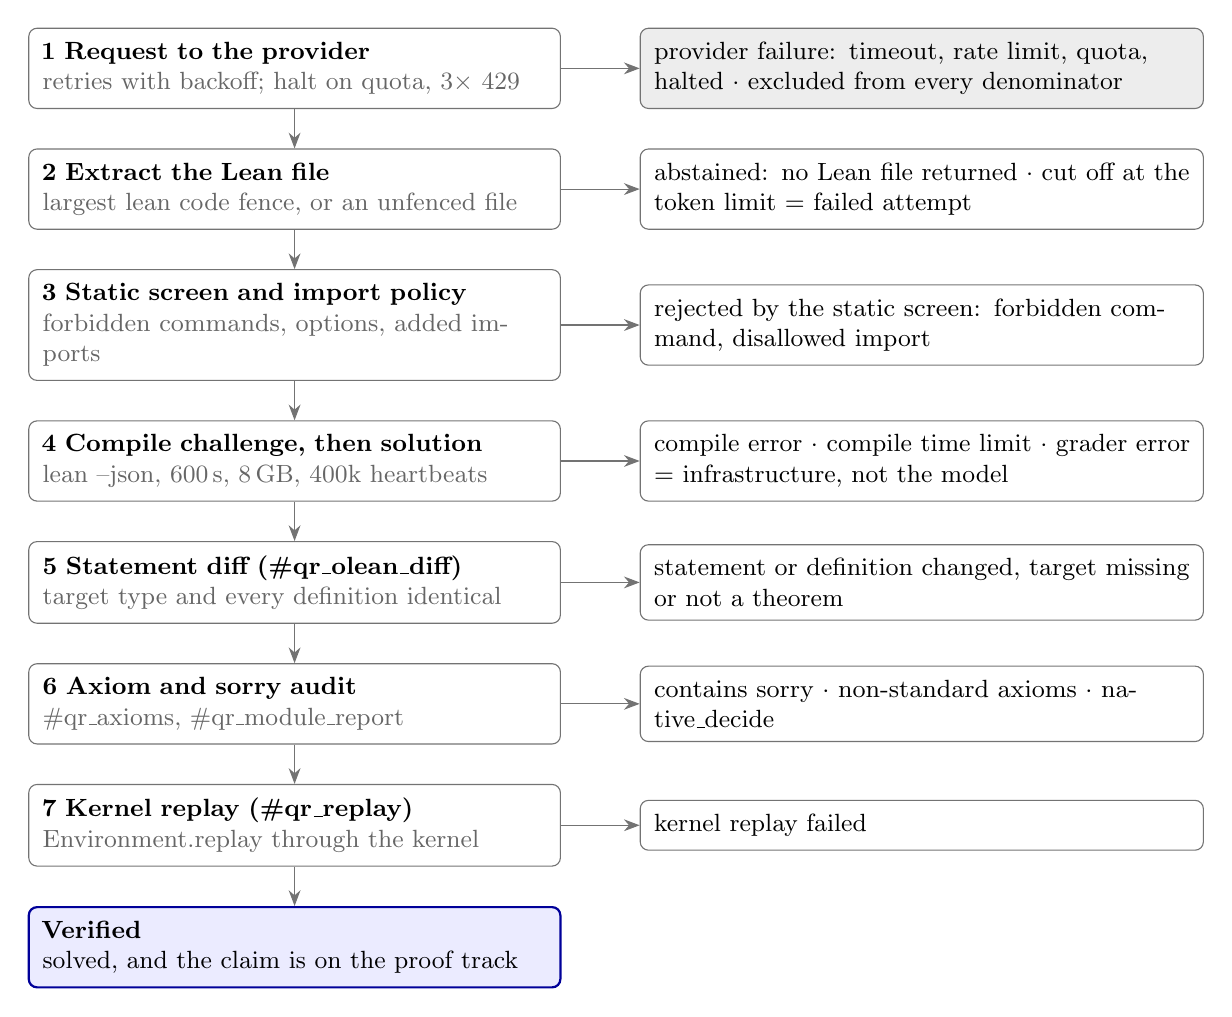
\begin{tikzpicture}[
  qrstep/.style={draw=black!55, rounded corners=3pt, align=left, text width=64mm, inner sep=5pt, font=\small},
  qrexit/.style={draw=black!55, rounded corners=3pt, align=left, text width=68mm, inner sep=5pt, font=\small},
  qrinfra/.style={qrexit, fill=black!7},
  qrok/.style={qrstep, fill=blue!8, draw=blue!60!black, thick},
  >={Stealth[length=2mm]}, node distance=5mm and 10mm]
\node[qrstep] (s1) {\textbf{1 Request to the provider}\\ {\color{black!60}retries with backoff; halt on quota, $3\times$ 429}};
\node[qrstep, below=of s1] (s2) {\textbf{2 Extract the Lean file}\\ {\color{black!60}largest \code{lean} code fence, or an unfenced file}};
\node[qrstep, below=of s2] (s3) {\textbf{3 Static screen and import policy}\\ {\color{black!60}forbidden commands, options, added imports}};
\node[qrstep, below=of s3] (s4) {\textbf{4 Compile challenge, then solution}\\ {\color{black!60}\code{lean --json}, 600\,s, 8\,GB, 400k heartbeats}};
\node[qrstep, below=of s4] (s5) {\textbf{5 Statement diff (\code{\#qr\_olean\_diff})}\\ {\color{black!60}target type and every definition identical}};
\node[qrstep, below=of s5] (s6) {\textbf{6 Axiom and sorry audit}\\ {\color{black!60}\code{\#qr\_axioms}, \code{\#qr\_module\_report}}};
\node[qrstep, below=of s6] (s7) {\textbf{7 Kernel replay (\code{\#qr\_replay})}\\ {\color{black!60}\code{Environment.replay} through the kernel}};
\node[qrok, below=of s7] (s8) {\textbf{Verified}\\ solved, and the claim is on the proof track};
\node[qrinfra, right=of s1] (e1) {provider failure: timeout, rate limit, quota, halted $\cdot$ excluded from every denominator};
\node[qrexit, right=of s2] (e2) {abstained: no Lean file returned $\cdot$ cut off at the token limit = failed attempt};
\node[qrexit, right=of s3] (e3) {rejected by the static screen: forbidden command, disallowed import};
\node[qrexit, right=of s4] (e4) {compile error $\cdot$ compile time limit $\cdot$ grader error = infrastructure, not the model};
\node[qrexit, right=of s5] (e5) {statement or definition changed, target missing or not a theorem};
\node[qrexit, right=of s6] (e6) {contains \code{sorry} $\cdot$ non-standard axioms $\cdot$ \code{native\_decide}};
\node[qrexit, right=of s7] (e7) {kernel replay failed};
\foreach \i/\j in {1/2,2/3,3/4,4/5,5/6,6/7,7/8} \draw[->, black!55] (s\i) -- (s\j);
\foreach \i in {1,...,7} \draw[->, black!55] (s\i) -- (e\i);
\end{tikzpicture}
\caption{One prove attempt: seven checks, seven exits, one success. The first exit (tinted) is a failure of the infrastructure and leaves every denominator; from the second exit on, the attempt counts against the model. A grader error at step~4 is also infrastructure.}
\label{fig:attempt}
\end{figure}

\begin{table}[htbp]
\centering\small
\caption{Stages of a run.}
\label{tab:stages}
\begin{tabular}{L{20mm}L{96mm}L{36mm}}
\toprule
Stage & What happens & Written \\
\midrule
discovery & the corpus is fetched from GitHub or a local path at the pinned ref; the resolved commit is locked, and a later stage aborts if the repository's commit has moved & \code{manifest.json} \\
preparation & \emph{prove}: the challenge file \code{challenge\_\_main\_theorem.lean} is copied and any file whose \code{sorry} count is not 1 is flagged. \emph{formalize}: PDF passages are extracted, a definitions-only prelude is built with \code{lake build}, the reference statement is audited and compiled as its own module, and a per-target context is assembled; a leak guard rejects any prompt that contains reference proof text & \code{prepared/<paper>/} \\
generation & one request per attempt, prompt template \code{qedrank-prove-v1} or \code{qedrank-prompt-v2}; the prove loop runs attempt $\to$ problem $\to$ provider, so attempt~1 of every problem exists before attempt~2 starts (the formalize loop is paper $\to$ target $\to$ provider $\to$ attempt); before each live request the grader compiles the challenge itself, and a challenge that does not compile is recorded as an infrastructure failure, never charged to the model & \code{items/<key>/response-a\{k\}r\{r\}.txt}, generation record \\
compilation & the model's whole file (no splicing) is extracted from the largest \code{lean} code fence, an unfenced file is accepted, no file is an abstention; the static screen and import policy run first; then \code{lean --json -M 8192 -DmaxHeartbeats=400000} is spawned directly with the project's \code{LEAN\_PATH}, 600\,s per file, two files at a time by default, and \code{*\_API\_KEY}/\code{GITHUB\_TOKEN} removed from its environment & \code{.olean}, compiler output \\
audit & \code{\#qr\_olean\_diff} compares the challenge's and the submission's object files: the target's type and every non-theorem declaration must be identical; \code{\#qr\_axioms} (via \code{collectAxioms}) and \code{\#qr\_module\_report} find non-standard axioms and \code{sorry} in each declaration; \code{\#qr\_replay} re-checks the environment through the kernel & \code{grade} block of the item \\
comparison & \emph{formalize} only: Part~A is stripped of proofs and compiled in namespace \code{QRModel}; the statement-fidelity check of Section~\ref{sec:controls} compares it with the audited reference; Part~B is compiled unchanged and its target checked for A/B consistency with \code{\#qr\_compare} & \code{comparison}, \code{statement\_match} \\
statistics & item records are aggregated into results and the summary, with the paper-cluster bootstrap of Section~\ref{sec:metrics}; exports for the app & \code{results.json}, \code{summary.json}, \code{exports/items.json}, \code{progress.json} \\
\bottomrule
\end{tabular}
\end{table}

\paragraph{Item record} (\code{items/\allowbreak <paper>\_\_\allowbreak <target>\_\_\allowbreak <provider>/\allowbreak attempt-a\{k\}r\{r\}.json}, schema \code{qedrank-item-v1}). It holds the generation (provider, model id, host, response model, finish reason, provider attempts and retry waits, usage in input / output / reasoning / cached tokens, observed latency including retries and working time of the successful request, the sampling actually sent, prompt hash and template version), the parse result, the static-screen and compile results, the audit, the statement match, timing, eligibility, the five outcome flags (\code{infrastructure\_failure}, \code{compiled}, \code{audit\_clean}, \code{statement\_faithful}, \code{verified}) and free-text notes such as \code{output\_truncated}, \code{multiple\_blocks\_largest\_used}, \code{no\_answer\_within\_output\_budget} or \code{ESCALATE} (an apparent proof of an open claim). A grader error turns the item into an infrastructure failure. Cost is not stored per item; it is computed at summary time from the pricing table.

\paragraph{Run record} (\code{run.json}, schema \code{qedrank-run-v1}): run id, source request and resolved commit with date, models with their hosts and facts, protocol (\code{single\_call} or \code{agent}), task, harness commit with branch, dirty flag and changed files, prompt template version, system prompt, machine, the full effective config, stage records with counters (total, done, skipped, halted, generated, generation failed, compiled, verified, infrastructure, errors), provider halts, re-evaluations and wall-clock time. \code{resume} rebuilds the config in the order defaults $<$ stored config $<$ \code{--config} file $<$ flags, restores the Lean project, skips completed attempts unless \code{--reevaluate}, and retries infrastructure failures with \code{--retry-failed}; pricing and bootstrap settings always come from the current config.

\paragraph{Agent protocol.} QEDRank also contains its own Inspect~AI harness (\code{harness/}: sandboxed agent, at most $x$ sessions joined by a \code{HANDOFF.md}, QEDRank's \code{grade} after every session) whose Docker image is still untested, and the \code{import-agent} command, which turns an agent bundle, from that harness or from the ProofBench team's, into a run with protocol \code{agent} so the same statistics apply.

% ------------------------------------------------------------------
\section{Models, providers and sampling}

Two models have been run so far; the roster has eleven default slots behind one call path, so a further model is a configuration entry, not code. All slots except the Anthropic ones speak the OpenAI-compatible chat protocol, which is also what vLLM and llama.cpp serve (Table~\ref{tab:roster}).

\begin{table}[htbp]
\centering\small
\caption{Model roster.}
\label{tab:roster}
\begin{tabular}{L{22mm}L{48mm}L{34mm}L{44mm}}
\toprule
Slot & Model id & Host & Request shape \\
\midrule
\code{qwen} & \code{qwen3-30b-a3b-instruct-2507} (30.5\,B parameters, 3.3\,B active, released 2025-07-30) & \code{chat-ai.academiccloud.de/v1}; a base-URL override points it at a self-hosted server & \code{temperature}, and \code{top\_p}, \code{top\_k}, \code{presence\_penalty} when configured; \code{max\_tokens} \\
\code{kimi} & \code{kimi-k3} (2.8\,T parameters, 104\,B active, released 2026-07-16) & \code{api.moonshot.ai/v1} & no temperature (the provider sets it); \code{reasoning\_effort} low, high or max; the model always reasons, and reasoning tokens count against \code{max\_tokens} \\
\code{fable}, \code{opus} & \code{claude-fable-5-1}, \code{claude-opus-5-5} & Anthropic Messages & \code{output\_config.effort}, no temperature \\
\code{gpt6\_astra}, \code{gpt6\_sol}, \code{gpt56\_terra}, \code{gpt54} & \code{gpt-6-astra}, \code{gpt-6-sol}, \code{gpt-5.6-terra}, \code{gpt-5.4} & \code{api.openai.com/v1} & \code{max\_completion\_tokens} and \code{reasoning\_effort}, no temperature \\
\code{llama}, \code{mistral}, \code{deepseek} & \code{meta-llama-3.1-8b-instruct}, \code{labs-leanstral-2603}, \code{deepseek-v4-pro} & GWDG, Mistral, DeepSeek & temperature sent \\
optional & any OpenAI-compatible endpoint (\code{custom}, OpenRouter, Together, Groq, NVIDIA, Hugging Face, Gemini) & by configuration & as above \\
\bottomrule
\end{tabular}
\end{table}

\paragraph{Sampling.} Single-attempt runs use temperature 0 where the provider allows it. Pass@$k$ needs temperature above 0; the Qwen3-2507 model card recommends 0.7 with top-p 0.8, top-k 20 and a presence penalty of 0--2, which \code{configs/qwen-prove-pass8.json} adopts. Whatever is sent is recorded in the generation's \code{sampling} field and in \code{summary.settings} (temperature, top\_p, top\_k, presence\_penalty, effort, max\_tokens). An environment variable \code{QEDRANK\_EFFORT\_<slot>} can override the configured effort for one run.

\paragraph{Retries, quota and halts.} HTTP 408, 425, 429, 5xx and network errors are retried (4 times by default, 6 in the pass@8 configs) with delay $\min(\text{max},\ \text{Retry-After or base}\cdot 2^{a-1} + \text{jitter})$; for 429 the wait is never shorter than the exponential term. A 429 whose body reports an exhausted balance becomes \code{insufficient\_quota} and is not retried. Three consecutive rate-limit failures, or one quota failure, halt the provider for the rest of the process: later requests return \code{halted} without being sent and leave no item record, so the run can be resumed with \code{--retry-failed} once the account is restored. Error kinds: \code{not\_configured}, \code{retired}, \code{http\_error}, \code{rate\_limited}, \code{insufficient\_quota}, \code{timeout}, \code{network}, \code{empty\_response} (finish reason \code{length} with no text), \code{refusal}, \code{provider\_error}, \code{halted}, \code{challenge\_does\_not\_compile}.

\begin{table}[htbp]
\centering\small
\caption{Prepared pass@8 configurations.}
\label{tab:configs}
\begin{tabular}{L{60mm}L{44mm}L{44mm}}
\toprule
Setting & \code{kimi-prove-pass8.json} & \code{qwen-prove-pass8.json} \\
\midrule
attempts & 8 & 8 \\
effort / temperature & max / provider default & --- / 0.7, top-p 0.8, top-k 20 \\
max output tokens & 65,536 & 16,384 \\
request timeout & 2,700\,s & 600\,s \\
retries, base, max delay & 6, 15\,s, 120\,s & 6, 15\,s, 120\,s \\
requests in flight per provider / items / Lean & 8 / 16 / default & 3 / 8 / 3 \\
pricing (USD per M tokens, input / output) & 3 / 15 & none (academic endpoint) \\
\bottomrule
\end{tabular}
\end{table}

\paragraph{What is recorded per request.} Provider, model id, host, the model name the server reports, finish reason, number of provider attempts and total retry wait, input / output / reasoning / cached tokens, observed latency including retries, working time of the successful request, the sampling sent, prompt hash and template version. Cost is computed at summary time as input tokens $\times$ input price plus output tokens $\times$ output price, with prices keyed by model id.

% ------------------------------------------------------------------
\section{Metrics and statistics}
\label{sec:metrics}

Every rate is a fraction num\,/\,den over eligible items, reported with its denominator; \code{summary.json} carries bootstrap intervals, the LaTeX matrices Clopper--Pearson intervals, and both say which.

\paragraph{Rates per model and target} (\code{by\_target[target][model]}): \code{statement\_faithful}, \code{compile}, \code{audit\_clean}, \code{verified\_pass1}, \code{abstention}, \code{unresolved}, \code{timeout}; distributions of time (observed model latency, Lean time, total item time), tokens, lines of code; \code{cost}; \code{calibration}. Each rate field holds \code{num}, \code{den}, \code{value}, \code{ci\_lo}, \code{ci\_hi}, \code{ci\_method}, \code{ci\_B}.

\paragraph{Intervals.} The summary uses a percentile bootstrap \cite{efron1979} that resamples \emph{paper ids} with replacement, so all targets, models and attempts of one paper move together: $B = 2{,}000$, seed 20260930 (mulberry32), $\alpha = 0.05$, bounds null when fewer than 10 finite draws exist. The LaTeX generators and the benchmark comparison use the exact two-sided 95\,\% Clopper--Pearson interval \cite{clopper1934}, found by bisection on the binomial distribution; it treats items as independent and is the conventional interval for a benchmark table.

\paragraph{pass@$k$.} For an item with $n$ attempts of which $c$ succeeded, the unbiased estimator of Chen et al.\ \cite{chen2021} is
\begin{equation}
\operatorname{pass@}k \;=\; 1 - \frac{\binom{n-c}{k}}{\binom{n}{k}} \;=\; 1 - \prod_{i=n-c+1}^{n}\Bigl(1 - \frac{k}{i}\Bigr),
\end{equation}
computed as the product for numerical stability; it is undefined (null) when $n < k$ and 1 when $n - c < k$. The curve is reported at $k = 1, 2, 4, \dots$ up to $n$ and at $n$ itself, each point with \code{items}, \code{items\_short} (items with fewer than $k$ attempts, which are left out of that point), \code{items\_solved\_any} and a bootstrap interval. The pool is the pass@1 setting, repair round~0, no infrastructure failure, proof track. The summary also gives the mean success per attempt, the per-attempt rates and their standard deviation across attempts, so a drift between attempt~1 and attempt~8 (a provider that degrades, a cache that warms) is visible.

\paragraph{Model comparison} on the papers all models share: Cochran's $Q$ \cite{cochran1950} across models, exact McNemar tests \cite{mcnemar1947} for each pair with Holm correction \cite{holm1979}, a paired bootstrap of the difference, and a descriptive ranking by point estimate; only pairs listed as \emph{statistically supported} are called different. No weighted composite score is computed.

\paragraph{Calibration.} The two confidences of the formalize task (statement faithful, proof passes) are scored by root-mean-square error over 10 bins against the observed rate, with the abstention rate beside it.

\paragraph{Cost.} Input tokens$/10^6 \times$ input price $+$ output tokens$/10^6 \times$ output price per item, summed per model, and divided by the number of verified successes for \emph{cost per verified success}; \code{n\_priced} says how many items had a price.

\paragraph{Counting rules.}
\begin{itemize}
\item A provider failure (timeout, rate limit, quota, halt) or a grader error is an infrastructure failure: excluded from every denominator and counted separately.
\item An answer cut off at the output limit, including one whose budget was spent on reasoning with no visible text, is a failed attempt of the model.
\item An abstention (no Lean file) is a failure in the proof track and is also reported as a rate of its own.
\item A compiling file with \code{sorry}, a changed statement, a non-standard axiom or a failed kernel replay is \emph{compiled} but not \emph{verified}.
\item Open and uncertain claims are counted in the statement track only; an apparent proof of one is flagged \code{ESCALATE} for human audit and does not enter \code{verified}.
\end{itemize}

% ------------------------------------------------------------------
\section{Validity controls}
\label{sec:controls}

Each control below exists because its absence was observed to bias a run at least once; Section~\ref{sec:runs} records the incidents.

\paragraph{Corpus and prompt integrity.}
\begin{itemize}
\item The corpus commit is resolved at discovery and locked; a later stage aborts if the repository has moved.
\item The formalize prompt passes a leak guard that rejects any text found in a reference proof; the prove prompt contains the challenge file and nothing else from the repository.
\item Before a live request, the grader compiles the challenge file itself; a challenge that does not compile in the grader is an infrastructure failure, not a model failure.
\end{itemize}

\paragraph{Provider failures kept apart from model outcomes.}
\begin{itemize}
\item Timeouts, rate limits, exhausted quota and halts are their own error kinds and never enter a denominator.
\item A provider is halted after one quota error or three consecutive rate-limit errors; halted items are left unrecorded so that \code{resume --retry-failed} fills them later and a throttled run cannot yield a score.
\item Attempt-major order in the prove task: attempt~1 of every problem exists before attempt~2 begins, so a run stopped early is a complete pass@1 run rather than a biased pass@$k$ sample.
\end{itemize}

\paragraph{Grader strictness.}
\begin{itemize}
\item Static screen: file size above 512\,KiB, \code{prelude} or module headers, forbidden commands (\code{\#eval}, \code{\#exit}, \code{run\_cmd}, \code{run\_elab}, \code{run\_tac}, \code{initialize}, \code{elab}, \code{macro}, \code{syntax}, \code{implemented\_by}, \code{extern}, \code{unsafe}, \dots), the option \code{debug.skipKernelTC}, heartbeat caps above the grader's.
\item Import policy: the challenge's own imports are always allowed; added imports must start with Mathlib, Std, Lean, Init, Aesop, Batteries, Qq, ProofWidgets, Plausible, LeanSearchClient, ImportGraph or \code{ProofBench.Mathlib\_Problems}; \code{ProofBench.Mathlib}, \code{ProofBench.PROBLEMS} and \code{ProofBench.DATABASE} are never allowed; dropping a challenge import is a rejection.
\item Object-file diff of the target's type and every non-theorem declaration, \code{collectAxioms} against the allowed set, a per-declaration \code{sorry} report, and a kernel replay of the whole environment.
\item Resource caps per compile (600\,s, 8\,GB, 400,000 heartbeats) and an environment stripped of API keys and the GitHub token.
\end{itemize}

\paragraph{Protocol stability.}
\begin{itemize}
\item \code{resume} restores generation, Lean, grading and concurrency settings from \code{run.json}; the model list comes from the run's selection and the task from the run.
\item Every run records the harness commit and whether the working tree was dirty, the prompt template version, the system prompt and the machine; the ProofBench harness freezes the same in \code{manifest.json}.
\item Re-evaluations with a changed grader are appended to \code{run.reevaluations}, so a re-grade is visible, not silent.
\end{itemize}

\paragraph{Statement fidelity (formalize, Part A).} The model's statement and the audited reference are compiled as separate modules and compared by \code{\#qr\_compare} at syntactic, reducible and default transparency; if not definitionally identical, both implications are attempted with a tactic portfolio (\code{exact}, \code{simpa}, \code{simp\_all}, \code{aesop}, \code{omega}, \code{exact?}, optionally \code{unfold \dots; aesop}), each proof must use its hypothesis, and neither statement may be provable outright. Outcomes: \code{definitionally\_identical}, \code{equivalent}, \code{unresolved}, \code{not\_evaluated}; \code{stronger}, \code{weaker}, \code{different} and \code{expert\_confirmed\_equivalent} come only from a human decision file (\code{review/decisions.json}). Accepted matches are the first two and the expert-confirmed one. An \code{unresolved} item is a question for an expert, never evidence of a mistranslation.

\paragraph{Related tool, not part of QEDRank.} \code{QED\_LEAF} (\code{qed-leaf equiv}, \code{qed-leaf fidelity-bench}, PR~\#2 of 2026-10-11) tests the opposite risk, that an equivalence checker accepts a wrong statement: it uses logic-level tactics only, because any two true closed statements are provable from each other, and takes ground truth from mutants that are refuted. On 24 core-Lean theorems with 279 variants it raised 0 of 96 false alarms on rewordings (against 96 for a structural and 57 for a definitional-equality check) and flagged all 93 refuted mutants. It has not yet been run against ProofBench's Mathlib project.

\paragraph{Human audit.} Apparent proofs of open claims (\code{ESCALATE}) and every agent solve are reviewed by hand; a \code{review/audit.json} can reject a solve after the fact.

% ------------------------------------------------------------------
\section{The agent harness (proofbench-eval-apptainer)}
\label{sec:harness}

The ProofBench team's harness gives every model the same agent loop, tools, sandbox and budgets, and grades with Lean alone. It was copied from \code{proof-bench/proofbench-eval-apptainer} main (\code{2803e81}, 51 commits) to branch \code{DGX\_Testing} of \code{vaibhav-baj/QEDRank} on 2026-10-13, and set up at \code{C:\textbackslash proofbench-eval} on the PC.

\paragraph{Agent.} An Inspect~AI \cite{inspect} ReAct \cite{yao2023} agent with \code{bash}, \code{python}, a text editor and \code{lean-lsp-mcp} (Lean language server as tools), optionally a web-search tool (off in all runs so far). The sandbox is a Docker container built from the pinned toolchain, the Mathlib cache, only the statement modules the selected problems import, and offline helpers (sympy, networkx, python-sat, SageMath 10.9 with GAP and nauty, CaDiCaL 1.7.3). The container has no network and no API key; the model never sees the proctor library.

\begin{table}[htbp]
\centering\small
\caption{Budgets (defaults of \code{scripts/run.sh}).}
\label{tab:budgets}
\begin{tabular}{L{100mm}L{40mm}}
\toprule
Limit & Value \\
\midrule
Sessions per problem, chained by a handoff note & 10 \\
Output tokens per session, reasoning included & 30,000 \\
Total tokens per session & 1,000,000 \\
Working time per session & 1,800\,s \\
Output tokens for the handoff note & 8,000 \\
Tokens per model reply & 16,000 \\
Request timeout / single attempt & 1,800\,s / 600\,s \\
Wall clock per problem (sessions $\times$ working time $\times$ 3) & 54,000\,s \\
Problems in parallel & 4 (2 on the PC) \\
Epochs & 1, fixed: a problem is never restarted from scratch \\
\bottomrule
\end{tabular}
\end{table}

\paragraph{Grading} runs in a second \code{verifier} container the agent never touched; only the submission's source text crosses over. Layer~1, \code{check\_proof.py}: statement unchanged, imports limited to Mathlib and the statement layer, no \code{sorry} or \code{axiom} in any file, helper files under \code{Submission/} build, main file compiles, axioms limited to \code{propext}, \code{Classical.choice}, \code{Quot.sound}; it also refuses \code{\#} commands, \code{initialize}/\code{run\_cmd}, kernel-skipping options and notation or scope changes ahead of the statement. Layer~2, Comparator \cite{comparator} (Lean FRO): rebuilds statement and submission in a Landlock \cite{landlock} sandbox (\code{landrun}), requires identical statements and dependencies, replays the proof through the kernel via \code{lean4export} \cite{lean4export}, and checks the axioms.

\paragraph{Outputs.} \code{manifest.json} freezes harness commit, image id, Lean toolchain, ProofBench commit, model, effort, search, network, epochs and all limits; \code{scripts/analyze.py} writes \code{results.csv} with, per problem: \code{correct}, \code{sessions\_used}, \code{session\_ends} (submit, token, working, error), tokens in/out/total, total and working time, tool calls and errors, model calls, proof lines, compile seconds, axioms. Inspect reports accuracy $\pm$ standard error over the problems of a run.

\paragraph{Verification on the PC (2026-10-13).} The P110 reference solution passed both layers (``Your solution is okay!''); a file that leaves the \code{sorry} was rejected (\code{sorryAx}). Image checks: Lean 4.33.1, P109 compiles, \code{lean-lsp-mcp} answers, verifier binaries present, Landlock engages in best-effort mode under WSL2.

\paragraph{Relation to QEDRank.} \code{correct = 1} corresponds to QEDRank's \emph{verified}; the harness measures one agentic attempt per problem, so pass@$k$ is not defined for it, and provider failures appear as \code{session\_ends = error} rather than as a separate class. QEDRank's \code{import-agent} command reads Inspect logs into its item-record format so that the same statistics and LaTeX tables can be produced for agent runs.

% ------------------------------------------------------------------
\section{Infrastructure}
\label{sec:infra}

The limiting resource was never compute but access: rate limits on hosted APIs, two-factor logins on the HPC, and GPU generations too old for current serving software. Four environments were used (Table~\ref{tab:infra}).

\begin{table}[htbp]
\centering\small
\caption{Environments.}
\label{tab:infra}
\begin{tabular}{L{28mm}L{26mm}L{38mm}L{56mm}}
\toprule
Environment & Role & What worked & What failed, and the fix \\
\midrule
Windows 11 PC, Docker Desktop (WSL2 kernel 6.18, Landlock ABI v7), Git Bash & runs QEDRank (CLI, run server, app) and the agent harness & both harnesses end to end; Lean compiles in 30\,s--5\,min per file & Python defaults (cp1252, CRLF) corrupted \code{lake-manifest.json} and \code{modules.txt} in the image build: fixed with \code{PYTHONUTF8=1} and explicit \code{encoding}/\code{newline} in \code{build\_image.sh} (patch not yet upstreamed); Git Bash rewrote \code{/opt/\dots} paths: \code{MSYS\_NO\_PATHCONV=1} \\
GWDG Chat AI (\code{chat-ai.academiccloud.de}, OpenAI-compatible) \cite{gwdg} & hosted open-weight models & \code{qwen3-30b-a3b-instruct-2507} reliable, tool calls correct & key limits 30/min, 200/h, 1,000/day, 3,000/month make an agent run (hundreds of calls per problem) impractical; \code{qwen3.8-27b} returned HTTP 500 on tool calls; served precision not documented \\
TU Freiberg HPC (\code{llogin01}, Slurm, partition \code{gpu32long}, NVIDIA RTX PRO 5000 Blackwell 48\,GB) & self-hosted vLLM \cite{kwon2023} server for Qwen3-30B-A3B in BF16 & vLLM 0.31.0 in a venv on system Python 3.12; job 6847 on 2 GPUs reached \emph{Application startup complete} with 131k context and the \code{hermes} tool parser & compute nodes lack \code{Python.h}, so Triton's JIT compile failed: fixed by pointing \code{CPATH} at headers from a \code{uv}-managed CPython 3.12 in \code{\$SCRATCH}; every login needs password + 2FA, port 22 to GitHub is blocked (\code{ssh.github.com:443}); the HPC-native sandbox needs the private \code{inspect-apptainer} package, not available to this account \\
DGX-2 (\code{dgx-2}, Ubuntu 22.04, kernel 5.15, 16 $\times$ Tesla V100 32\,GB, shared) & run model server and harness on one machine, no tunnel, no PC & Docker with GPUs as an unprivileged user; \code{/raid/mitarbeiter/<user>} for the 61\,GB model; \code{tmux} & \code{vllm/vllm-openai:latest} (torch 2.13, CUDA 13) has no \code{sm\_70} kernels: ``no kernel image is available''; llama.cpp \cite{llamacpp} built from \code{ceefd16} with CUDA 12.8 for arch 70 answered a tool-call test with Qwen3-0.6B (GPU use still to be confirmed); V100 has no BF16, so the model runs in FP16; Python 3.10 is below the harness's 3.11 minimum (\code{uv} Python 3.12) \\
\bottomrule
\end{tabular}
\end{table}

\paragraph{Moonshot (Kimi K3).} Tier~0 allows 1 concurrent request, 3 requests per minute and 1.5\,M tokens per day; Tier~1 (\$10 cumulative top-up) allows 15 concurrent requests with no daily cap. Price \$3 / \$15 per million input / output tokens. The model always reasons; \code{reasoning\_effort} is low, high or max. Open weights exist (K3 1.56\,TB MXFP4; K2.5 and K2-Thinking 595\,GB INT4) but exceed every GPU budget available here.

\paragraph{Serving routes compared.} The hybrid route (vLLM on the HPC, harness on the PC through \code{ssh -N -L 8000:<node>:8000}) works but needs three open terminals and two 2FA logins per run. The DGX route needs one login and survives disconnects, at the price of FP16 and a different server program; runs are labelled with the server, precision and version (\code{selfhosted-bf16-vllm0.31.0}, \code{fp16-llamacpp-<commit>}) so that the paper can report them apart.

% ------------------------------------------------------------------
\section{The QEDRank application}
\label{sec:app}

The web app is the operator's console: it freezes a corpus, starts and watches runs, and renders the summary a run produced. It computes no statistic itself (the Evaluation page states ``Nothing is computed here''); every number on screen is read from \code{summary.json}, so a figure in the app and a table in the paper come from the same file. Figure~\ref{fig:arch} shows the parts; Table~\ref{tab:pages} the six pages and Table~\ref{tab:evalpage} the sections of the Evaluation page.

\begin{figure}[htbp]
\centering
\resizebox{\linewidth}{!}{%
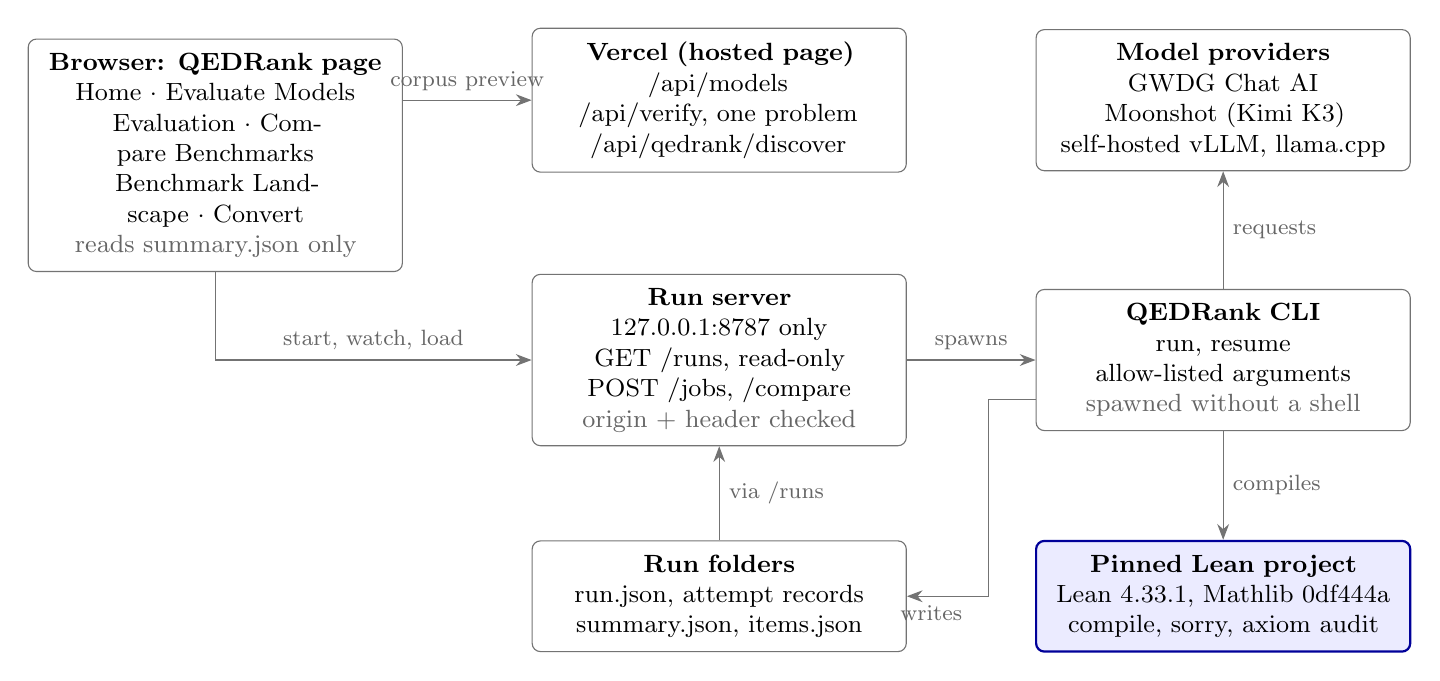
\begin{tikzpicture}[
  qrbox/.style={draw=black!55, rounded corners=3pt, align=center, text width=44mm, inner sep=5pt, font=\small},
  qrmain/.style={qrbox, fill=blue!8, draw=blue!60!black, thick},
  qrlab/.style={font=\footnotesize, text=black!60},
  >={Stealth[length=2mm]}]
\node[qrbox] (browser) at (0,0) {\textbf{Browser: QEDRank page}\\ Home $\cdot$ Evaluate Models\\ Evaluation $\cdot$ Compare Benchmarks\\ Benchmark Landscape $\cdot$ Convert\\ {\color{black!60}reads summary.json only}};
\node[qrbox] (vercel) at (6.4,0.7) {\textbf{Vercel (hosted page)}\\ /api/models\\ /api/verify, one problem\\ /api/qedrank/discover};
\node[qrbox] (server) at (6.4,-2.6) {\textbf{Run server}\\ 127.0.0.1:8787 only\\ GET /runs, read-only\\ POST /jobs, /compare\\ {\color{black!60}origin + header checked}};
\node[qrbox] (folders) at (6.4,-5.6) {\textbf{Run folders}\\ run.json, attempt records\\ summary.json, items.json};
\node[qrbox] (providers) at (12.8,0.7) {\textbf{Model providers}\\ GWDG Chat AI\\ Moonshot (Kimi K3)\\ self-hosted vLLM, llama.cpp};
\node[qrbox] (cli) at (12.8,-2.6) {\textbf{QEDRank CLI}\\ run, resume\\ allow-listed arguments\\ {\color{black!60}spawned without a shell}};
\node[qrmain] (lean) at (12.8,-5.6) {\textbf{Pinned Lean project}\\ Lean 4.33.1, Mathlib 0df444a\\ compile, sorry, axiom audit};
\draw[->, black!55] (browser.east |- vercel.west) -- (vercel.west) node[qrlab, midway, above] {corpus preview};
\draw[->, black!55] (browser.south) |- (server.west) node[qrlab, pos=0.75, above] {start, watch, load};
\draw[->, black!55] (server.east) -- (cli.west) node[qrlab, midway, above] {spawns};
\draw[->, black!55] (cli.north) -- (providers.south) node[qrlab, midway, right] {requests};
\draw[->, black!55] (cli.south) -- (lean.north) node[qrlab, midway, right] {compiles};
\draw[->, black!55] ($(cli.west)+(0,-0.5)$) -- ++(-0.6,0) |- (folders.east) node[qrlab, pos=0.85, below] {writes};
\draw[->, black!55] (folders.north) -- (server.south) node[qrlab, midway, right] {via /runs};
\end{tikzpicture}}
\caption{QEDRank architecture. Scores come from the local CLI and Lean; the hosted page only previews. The browser only starts jobs and reads files; the run server spawns the CLI with validated arguments, the CLI calls the providers and the pinned Lean project, and writes the run folder that the page reads back.}
\label{fig:arch}
\end{figure}

\begin{table}[htbp]
\centering\small
\caption{Pages of the app.}
\label{tab:pages}
\begin{tabular}{L{20mm}L{20mm}L{48mm}L{32mm}L{26mm}}
\toprule
Route & Page & What the operator does there & Data it reads & Role in testing \\
\midrule
\code{/} & Home & chooses one of the two workflows, Evaluate Models or Compare Benchmarks, each listed with what it measures & roster summary only & entry point; old links to the single-problem anchors are forwarded to Convert a Problem \\
\code{/benchmark} & Evaluate Models & step~0 picks models (with the masked key setup); step~1 \emph{Freeze and audit the corpus} (repo link, ref, subfolder, expected paper count $\to$ manifest with commit, paper table, target counts, flags); step~2 \emph{Run the benchmark from here} (task prove/formalize, targets, papers, run id, Lean project, dry run; Start, Stop, Load into Evaluation) or \emph{Load a run} (list, load, auto-refresh, or open files) & \code{POST /api/qedrank/discover}; run server \code{POST /jobs}, \code{GET /jobs/<id>?from=N}, \code{POST /jobs/<id>/stop}, \code{GET /runs}, \code{run.json}, \code{progress.json}, \code{summary.json}, \code{exports/items.json} & the only place a run is started from the page; shows the equivalent CLI command; the progress view counts generated / compiled / verified / infrastructure / error items live \\
\code{/evaluation} & Evaluation & reads a loaded run; downloads Summary JSON, Matrix CSV, Items JSON and a LaTeX report (metadata, models, result tables, item outcomes) & \code{summary.json}, \code{items.json} from session storage & the analysis console (Table~\ref{tab:evalpage}) \\
\code{/versus} & Compare Benchmarks & your benchmark (URL, ref, subfolder, optional token) against up to 7 benchmarks from \code{qedrank/data/benchmark-literature.json}; downloads JSON, Matrix CSV and LaTeX & run server \code{POST /compare} & produces the benchmark-comparison table and figures used in \code{paper/benchmark-comparison.tex} \\
\code{/compare} & Benchmark Landscape & ProofBench against the published Lean benchmarks: facts table, size against best reported success, statement complexity, subject heatmap, level composition, sources & \code{runs/\_compare/benchmark-comparison.json} (schema \code{qedrank-benchmark-comparison-v1}) or a file & positions the corpus relative to miniF2F \cite{zheng2022}, PutnamBench \cite{tsoukalas2024} and others for the related-work section \\
\code{/convert} & Convert a Problem & types one problem, sends it to every selected model with a key, rates the Lean output 1--5 & \code{POST /api/verify} (Vercel function), \code{POST /api/feedback} & model and key check before a run; correctness is not judged here \\
\bottomrule
\end{tabular}
\end{table}

\begin{table}[htbp]
\centering\small
\caption{Evaluation page: sections and the summary fields they read.}
\label{tab:evalpage}
\begin{tabular}{L{6mm}L{30mm}L{76mm}L{38mm}}
\toprule
\# & Section & Figure or table & Summary field \\
\midrule
-- & run bar and KPI tiles & run id, corpus commit, toolchain, harness commit, protocol, settings ($k$, temperature, max tokens, bootstrap $B$ and seed); best verified pass@1, papers, items, models, Cochran's $Q$, supported pairs & \code{run}, \code{settings}, \code{coverage}, \code{model\_comparison} \\
0 & Agent protocol (agent runs only) & solved within $k$ sessions, budgets, tool calls & \code{agent} \\
1 & Leaderboard & HBars of verified pass@1 with CI whiskers; GroupedBars of verified, statement faithful, compile, audit clean; one HBars per target; pass@$k$ GroupedBars when $k > 1$ & \code{by\_target[scope][model]}, \code{pass\_at\_k.curve} \\
2 & Heatmap & models $\times$ scopes, metric tab & \code{by\_target} \\
3 & Full matrix & 16-column MatrixTable with sandwich and paper-level columns; eligibility rules & \code{by\_target}, \code{paper\_level}, \code{eligibility\_rules} \\
4 & Statement matches & StackedBars of faithful / different / unresolved / not evaluated & \code{statement\_match\_counts} \\
5 & Time & RangeDots (median, IQR, p90) of model latency, Lean time, total item time & \code{time.*} \\
6 & Tokens and cost & GroupedBars of median input/output tokens; HBars of cost per verified success & \code{tokens.*}, \code{cost.per\_verified\_success\_usd} \\
7 & Calibration & Reliability diagram per model: stated confidence against observed rate, statement and proof audit & \code{calibration.statement}, \code{calibration.proof\_audit} \\
8 & $k$-model comparison & descriptive ranking, PairMatrix of row-minus-column percentage points with $\bullet$ for Holm $p < 0.05$, McNemar table & \code{model\_comparison} \\
9 & Subgroups & HBars per subject and per difficulty & \code{subgroups.by\_subject}, \code{by\_difficulty} \\
10 & Coverage & sandwich coverage, reference defects, subsets, caveats & \code{paper\_level}, \code{coverage}, \code{reference\_defects}, \code{caveats} \\
11 & Items & 8 filters plus search, per-item details, filtered CSV/JSON & \code{items.json} \\
\bottomrule
\end{tabular}
\end{table}

Every figure has a Chart/Table toggle, an Enlarge view and an error boundary (\code{ChartBoundary}) that shows the table if a chart throws; the Evaluation page went blank on the Kimi runs until the pair matrix learned to render an empty cell when two models share no graded paper.

\paragraph{Run server} (\code{node qedrank/cli.js serve}, or a double-click on \code{scripts\textbackslash serve.cmd}). It binds to 127.0.0.1:8787 and serves run folders read-only (\code{GET /runs}, \code{GET /runs/<id>/<file>}, file types limited to json, csv, txt, lean, md, pdf, with a path-traversal check). \code{POST /jobs} and \code{POST /compare} answer only to the app's own origins (localhost, \code{*.vercel.app}, or \code{--allow-origin}) with the header \code{X-QEDRank-Client}, accept at most 64\,KB, allow only \code{run} and \code{resume}, validate every argument against a regular expression or allow-list, spawn the CLI with an argument array (never a shell), run one job per run id, cap the log at 2\,MB, and stop a job with SIGTERM then SIGKILL after 5\,s. The GitHub token comes from \code{GITHUB\_TOKEN} or \code{gh auth token}, reaches the child process only and is never logged.

\paragraph{Deployment.} The page is hosted on Vercel (project \code{qedrank}); only the corpus preview and the single-problem bridge run there. Generation, Lean checking and evaluation always run on the operator's machine through the run server, which the deployed page reaches as a private-network request.

% ------------------------------------------------------------------
\section{Runs performed to date}
\label{sec:runs}

None of the runs in Table~\ref{tab:runs} is reportable as model performance; each row says why. Numbers come from the run folders' \code{summary.json} and the generated LaTeX matrices.

\begin{table}[htbp]
\centering\small
\caption{Runs to date.}
\label{tab:runs}
\begin{tabular}{L{26mm}L{14mm}L{32mm}L{38mm}L{36mm}}
\toprule
Run & Date & Task, corpus, models & Status & Key numbers \\
\midrule
\code{2026-10-11-466b32a} & 2026-10-11 & prove; 111 problems; Qwen3-30B-A3B (GWDG), Kimi~K3 (Moonshot); temperature 0, 16,384 tokens, 1 attempt & invalid grading: QEDRank's default Lean project (4.34.1) instead of the benchmark's; grader rejected imports that the challenge file itself contains & 48 Qwen + 2 Kimi answers failed with \code{unknown module prefix 'ProofBench'}; 11 Qwen answers wrongly rejected as \code{disallowed\_import} \\
\code{2026-10-11-466b32a-regrade} & 2026-10-12 & the same stored answers, re-graded in the pinned project (grader fix \code{5de6055}) & grading valid; Qwen numbers are a single-attempt baseline, Kimi's are not comparable & Qwen: 111 answered, 66 cut off at the token limit, 8/109 compiled, 7 of them with \code{sorry}, 1 with a changed statement, 0/80 verified. Kimi: 94/111 provider failures (37 timeouts at 300\,s, 57 HTTP 429), 15 abstentions, 2 graded, 0 verified \\
\code{2026-10-12-e631e6a} & 2026-10-12 & formalize; 28 papers $\times$ 3 targets; same models & reference statements prepared in the wrong project: 65/84 unavailable, 3 more lost to a QEDRank namespace-wrapper bug; only 16 main-theorem references; every prompt lacked the per-paper definitions & Kimi: 0 answers (14 HTTP 429, 70 refused for insufficient balance). Qwen: 0/77 statements compile, 35 cut off (30 of them repetition loops at temperature 0), 0/15 verified. Two counting bugs (comment-only proof files counted as compiled; non-existent Mathlib imports labelled infrastructure) are corrected in the LaTeX generator, not yet in the summary code \\
agent harness, GWDG & 2026-10-13 & prove, agent; P109--P111 at \code{0a4a476}; Qwen3-30B-A3B via GWDG & stopped after 14\,min at the user's request, 0 problems finished (200 requests/hour) & \code{manifest.json} records \code{harness\_dirty = true} (Windows build patch) \\
agent harness, self-hosted & 2026-10-13 & prove, agent; P109--P111; Qwen3-30B-A3B via HPC vLLM & aborted after 1\,min: the SSH tunnel was not open, every model call would have failed & none \\
Kimi~K3 pass@8 (\code{configs/kimi-prove-pass8.json}) & not started & prove; 111 problems; 8 attempts, effort max, 65,536 tokens, 45\,min timeout & waiting on: account top-up to Tier~1, a written no-training confirmation from Moonshot, and the decision whether to add hidden definitions to the prompt & estimated cost \$170--390 at effort max (pass@1 alone \$21--49); estimate, not measured \\
Qwen3 pass@8 (\code{configs/qwen-prove-pass8.json}) & not started & prove; 111 problems; 8 attempts at temperature 0.7, top-p 0.8, top-k 20 & live smoke test (2 problems $\times$ 2 attempts) passed end to end; waiting on the serving route & --- \\
\bottomrule
\end{tabular}
\end{table}

\paragraph{Lessons already applied.} The grader compiles the challenge file first and judges only imports a solution adds (\code{5de6055}). \code{resume} restores the stored generation, Lean, grading and concurrency settings, so a resumed run cannot silently change protocol. An answer cut off at the output limit is a failed attempt of the model, not an infrastructure failure. A provider is halted after exhausted quota or three consecutive rate-limit errors, and halted items stay unrecorded for \code{resume --retry-failed}, so a rate-limited run never produces a score.

% ------------------------------------------------------------------
\section{Threats to validity and limitations}
\label{sec:threats}

The two faults that invalidated the first runs were both in the measuring instrument, not in the models; the list below separates what has been fixed from what remains a limitation of the design.

\paragraph{Construct validity.}
\begin{itemize}
\item A compiling file is not a proof: 7 of Qwen's 8 compiling answers kept the \code{sorry}. Only kernel-replayed, axiom-checked, statement-unchanged files count. For formalize, an automated failure to prove two statements equivalent is not evidence that they differ; such items are \emph{unresolved} and need expert review.
\item The prove prompt contains the challenge file but not the definitions of the imported statement layer \code{ProofBench.Mathlib\_Problems}, which 52 of 111 problems use. Kimi declined those problems. Adding the definitions changes the protocol, so it must be decided before the pass@$k$ runs and applied to every model alike.
\end{itemize}

\paragraph{Internal validity.}
\begin{itemize}
\item Grading in the wrong Lean project and a too-strict import policy (fixed in \code{5de6055}, verified by re-grading with 0 grader errors).
\item 59\,\% of Qwen's answers were cut off at 16,384 output tokens, and at temperature 0 thirty formalize answers fell into repetition loops; the compile rate of such a run measures the budget as much as the model. Pass@$k$ configs use 16,384 tokens at temperature 0.7 for Qwen and 65,536 tokens for Kimi; the token limit is reported next to every rate.
\item Provider failures were 85\,\% of Kimi's pilot. They are excluded from denominators, but a model with few graded items has wide intervals and is not comparable; the provider-halt rule now stops a run instead of recording such items.
\item A resumed run could once change its settings; \code{resume} now restores them from \code{run.json}.
\end{itemize}

\paragraph{External validity.}
\begin{itemize}
\item One corpus of 111 problems clustered in papers; two models so far, both mixture-of-experts; the open-weight one is small (3.3\,B active parameters). Results will not generalise to frontier proprietary models without running them.
\item The same model is served three ways (GWDG, vLLM BF16, llama.cpp FP16) with different precisions and server programs; runs carry the route in their id and are reported separately.
\item The agent harness runs one attempt per problem and its sandboxes have reduced Landlock protection on WSL2 and on the DGX's 5.15 kernel; its \code{manifest.json} records \code{harness\_dirty = true} while the Windows build patch is unmerged.
\end{itemize}

\paragraph{Statistical conclusion validity.}
\begin{itemize}
\item Items are not independent; the summary's intervals come from a bootstrap that resamples papers, the LaTeX tables use binomial (Clopper--Pearson) intervals that ignore the clustering, and model comparisons use McNemar tests with Holm correction. Small denominators (8 eligible Kimi items) make most pairs unsupported.
\item The unbiased pass@$k$ estimator needs $n \geq k$ attempts per item; the summary reports the number of items with fewer attempts for each $k$.
\end{itemize}

\paragraph{Contamination.} Neither provider publishes a training cutoff and the corpus does not record publication dates, so exposure to the papers or to public formalizations cannot be assessed; solves of open problems are audited by hand.

% ------------------------------------------------------------------
\section{Ethics and data handling}

The corpus is private and partly unpublished, so every model call is a disclosure; the procedure limits what is disclosed, to whom, and under which terms.
\begin{itemize}
\item \textbf{Unpublished statements.} Problems are sent only to providers whose terms exclude training on API input, or to servers under the team's control. Moonshot (Kimi) has not yet given a written no-training confirmation; the Kimi runs stay blocked until it does. GWDG Chat~AI is operated by an academic computing centre; the self-hosted routes (HPC, DGX) disclose nothing outside the university.
\item \textbf{Proctor material.} Reference proofs, bounds and disproofs never enter a prompt or a sandbox image; the image builder refuses modules outside the statement layer, and QEDRank's prove prompt contains only the challenge file.
\item \textbf{Credentials.} API keys and the vLLM server key live in the user's environment or are read at a hidden prompt; they are never written to a tracked file, printed, or typed into a web page. The GitHub token comes from \code{gh auth token}. The run server binds to 127.0.0.1, answers job requests only to the app's own origins with a custom header, and runs an allow-list of commands with validated arguments, never a shell.
\item \textbf{Sandboxing.} Agent containers have no network and no host directories; grading runs in a second container as an unprivileged user; Comparator adds a Landlock sandbox (best-effort on WSL2 and on the DGX's 5.15 kernel, which are below the ABI level it was designed for).
\item \textbf{Shared hardware.} The DGX-2 is shared; GPU~8 was in use by another user during setup. The model (61\,GB) and images go to the group folder \code{/raid/mitarbeiter/<user>} and to Docker's store on \code{/raid}, which was 96\,\% full; the administrator should be told before full-size runs.
\item \textbf{Contamination.} Neither provider states a training cutoff and the problems' publication dates are not recorded in the corpus, so prior exposure cannot be assessed; this is reported as a caveat on every summary.
\end{itemize}

% ------------------------------------------------------------------
\section{Reproducibility}
\label{sec:repro}

A run is reproduced from its folder alone: \code{run.json} names the corpus commit, the harness commit, the Lean project and every setting; the item records hold the raw responses. Table~\ref{tab:where} lists the locations; the commands below are the ones used.

\begin{table}[htbp]
\centering\small
\caption{Locations.}
\label{tab:where}
\begin{tabular}{L{40mm}L{112mm}}
\toprule
Where & What \\
\midrule
\code{C:\textbackslash QEDRank} & the repository \code{github.com/vaibhav-baj/QEDRank}, branch \code{main}: one folder holding everything below \\
\code{QEDRank\_java/} & the app, the CLI (\code{node qedrank/cli.js}), the Lean audit project and \code{runs/} \\
\code{QEDRank-ProofBencheval/} & the agent harness (git subtree of \code{proof-bench/proofbench-eval-apptainer}, upstream \code{2803e81}, with the fork's fixes) with its \code{proofbench-statements} clone at \code{0a4a476}, image \code{proofbench-sandbox:latest} (P109--P111) \\
\code{proofbench-statements/} & the benchmark's pinned Lean project (Lean/Mathlib v4.33.1, all 185 modules built), used with \code{--lean-project}; not committed \\
\code{runs/<run-id>/} & \code{run.json}, \code{manifest.json}, \code{prepared/}, \code{items/<key>/attempt-a\{k\}r\{r\}.json} and \code{response-*.txt}, \code{results.json}, \code{summary.json}, \code{exports/items.json}, \code{progress.json} \\
\code{paper/} & \code{make-tex.cjs} (prove runs, $k \geq 1$) and \code{make-tex-formalize.cjs} (formalize, $k = 1$) regenerate every table and figure from a run folder; outputs \code{performance-matrix*.tex/.pdf}, \code{benchmark-comparison.tex} \\
\bottomrule
\end{tabular}
\end{table}

\begin{small}
\begin{verbatim}
# prove, 8 attempts, Qwen via the configured base URL, graded in the pinned project
node qedrank/cli.js run --repo https://github.com/proof-bench/proofbench-statements \
  --ref 466b32a --task prove --targets main_theorem --models qwen \
  --lean-project C:\proofbench-statements --config configs/qwen-prove-pass8.json \
  --run-id 2026-10-xx-466b32a-qwen-pass8
node qedrank/cli.js resume --run-id 2026-10-xx-466b32a-qwen-pass8 --retry-failed
node paper/make-tex.cjs runs/2026-10-xx-466b32a-qwen-pass8 \
  paper/performance-matrix-qwen-pass8.tex
npm test     # 87 passed, 1 skipped on 2026-10-13
             # (Lean fixture tests need QEDRANK_LEAN_TESTS=1)

# agent harness (Docker machine)
IDS="P109 P110 P111" scripts/build_image.sh
IDS="P109 P110 P111" MAX_SAMPLES=2 \
  MODEL=openai-api/qwen/qwen3-30b-a3b-instruct-2507 scripts/run.sh
python3 scripts/analyze.py logs/<RUN_ID>     # results.csv
\end{verbatim}
\end{small}

\paragraph{Frozen per run.} Corpus commit and date; harness commit, branch, dirty flag and changed files; Lean toolchain, Mathlib revision and lake options; prompt template version and system prompt; model ids and hosts; temperature, extra sampling, effort, max tokens, timeout, attempts, repair rounds, concurrency; bootstrap $B$ and seed; pricing used for cost. For the agent harness: image id, model, effort, search, network, epochs, sessions and all token and time limits.

\paragraph{Before the pass@$k$ runs} (open items found while writing this paper).
\begin{itemize}[label=\pending]
\item Commit the uncommitted harness changes, so that runs stop recording \code{harness.dirty = true}
\item Decide whether the prove prompt includes the definitions of \code{ProofBench.Mathlib\_Problems} (52 of 111 problems); apply to all models
\item Pass the pinned project's \code{leanOptions} (for example \code{maxSynthPendingDepth = 3}) in formalize compiles as \code{grade} already does
\item Fix \code{settings.primary\_endpoint} in \code{run.json}, which prints the formalize text for prove runs
\item Record \code{requests\_not\_sent} per halted provider rather than stage-wide
\item Align the web launcher's default task (\code{prove}) with the run server's default (\code{formalize})
\item Move the two formalize counting corrections (comment-only proof files; non-existent Mathlib imports) from the LaTeX generator into the summary code
\item Moonshot: Tier~1 top-up and a written no-training confirmation before any Kimi request with unpublished statements
\item DGX: confirm that llama.cpp uses the GPU, convert the official Qwen3-30B-A3B weights to FP16 GGUF, build the sandbox image, and label runs \code{fp16-llamacpp-<commit>}
\item Upstream the Windows \code{build\_image.sh} encoding patch to \code{proofbench-eval-apptainer}
\end{itemize}

% ------------------------------------------------------------------
\begin{thebibliography}{99}
\small
\bibitem{demoura2021} de Moura, L., Ullrich, S.: The Lean 4 Theorem Prover and Programming Language. In: Automated Deduction -- CADE 28, LNCS 12699, pp.~625--635. Springer (2021). doi:10.1007/978-3-030-79876-5\_37
\bibitem{mathlib2020} The mathlib Community: The Lean Mathematical Library. In: Proc.\ 9th ACM SIGPLAN Int.\ Conf.\ on Certified Programs and Proofs (CPP 2020), pp.~367--381 (2020). doi:10.1145/3372885.3373824
\bibitem{chen2021} Chen, M., Tworek, J., Jun, H., et al.: Evaluating Large Language Models Trained on Code. arXiv:2107.03374 (2021). (unbiased pass@$k$ estimator)
\bibitem{clopper1934} Clopper, C.~J., Pearson, E.~S.: The use of confidence or fiducial limits illustrated in the case of the binomial. Biometrika 26(4), 404--413 (1934)
\bibitem{efron1979} Efron, B.: Bootstrap methods: another look at the jackknife. Annals of Statistics 7(1), 1--26 (1979)
\bibitem{holm1979} Holm, S.: A simple sequentially rejective multiple test procedure. Scandinavian Journal of Statistics 6(2), 65--70 (1979)
\bibitem{mcnemar1947} McNemar, Q.: Note on the sampling error of the difference between correlated proportions or percentages. Psychometrika 12(2), 153--157 (1947)
\bibitem{cochran1950} Cochran, W.~G.: The comparison of percentages in matched samples. Biometrika 37(3/4), 256--266 (1950)
\bibitem{yao2023} Yao, S., Zhao, J., Yu, D., et al.: ReAct: Synergizing Reasoning and Acting in Language Models. In: ICLR 2023. arXiv:2210.03629
\bibitem{inspect} UK AI Security Institute: Inspect: an open-source framework for large language model evaluations (2024--). \url{https://inspect.aisi.org.uk}
\bibitem{qwen3} Qwen Team: Qwen3 Technical Report. arXiv:2505.09388 (2025)
\bibitem{qwen3card} Qwen Team: Qwen3-30B-A3B-Instruct-2507, model card (2025). \url{https://huggingface.co/Qwen/Qwen3-30B-A3B-Instruct-2507}
\bibitem{kimik2} Moonshot AI: Kimi K2: Open Agentic Intelligence. arXiv:2507.20534 (2025). $\dagger$
\bibitem{kimik3} Moonshot AI: Kimi K3, model card (2026). \url{https://huggingface.co/moonshotai/Kimi-K3}
\bibitem{kwon2023} Kwon, W., Li, Z., Zhuang, S., et al.: Efficient Memory Management for Large Language Model Serving with PagedAttention. In: Proc.\ 29th Symposium on Operating Systems Principles (SOSP 2023). (vLLM)
\bibitem{llamacpp} Gerganov, G., and contributors: llama.cpp: LLM inference in C/C++. \url{https://github.com/ggml-org/llama.cpp}, commit \code{ceefd16} (2026-10-16)
\bibitem{landlock} Sala\"un, M.: Landlock: unprivileged access control. Linux kernel documentation. \url{https://docs.kernel.org/userspace-api/landlock.html}
\bibitem{comparator} Lean FRO: Comparator: independent checking of Lean submissions against a challenge. \url{https://github.com/leanprover/comparator}
\bibitem{lean4export} Lean FRO: lean4export. \url{https://github.com/leanprover/lean4export}
\bibitem{leanlspmcp} lean-lsp-mcp: Lean language server as MCP tools. \url{https://github.com/oOo0oOo/lean-lsp-mcp} $\dagger$
\bibitem{zheng2022} Zheng, K., Han, J.~M., Polu, S.: miniF2F: a cross-system benchmark for formal Olympiad-level mathematics. In: ICLR 2022. arXiv:2109.00110
\bibitem{tsoukalas2024} Tsoukalas, G., Lee, J., Jennings, J., et al.: PutnamBench: Evaluating Neural Theorem-Provers on the Putnam Mathematical Competition. In: NeurIPS 2024 Datasets and Benchmarks. arXiv:2407.11214
\bibitem{improofbench} Schmitt, J., B\'erczi, G., Dekoninck, J., et al.: IMProofBench: Benchmarking AI on Research-Level Mathematical Proof Generation. arXiv:2509.26076 (2025). $\dagger$
\bibitem{kurtzer2017} Kurtzer, G.~M., Sochat, V., Bauer, M.~W.: Singularity: Scientific containers for mobility of compute. PLoS ONE 12(5), e0177459 (2017). (Apptainer's origin)
\bibitem{gwdg} GWDG / KISSKI: Chat AI, OpenAI-compatible API for hosted open-weight models. \url{https://chat-ai.academiccloud.de}
\bibitem{proofbench} ProofBench team: \code{proof-bench/proofbench-statements} (private statement corpus; commits \code{466b32a}, \code{0a4a476}) and \code{proof-bench/proofbench-eval-apptainer} (agent harness; commit \code{2803e81}). Private GitHub repositories (2026)
\bibitem{qedrank} This project: QEDRank, \code{vaibhav-baj/QEDRank}, branch \code{QEDRank} (evaluator, app, LaTeX generators) and branch \code{DGX\_Testing} (copy of the agent harness). Private GitHub repository (2026)
\end{thebibliography}

\noindent $\dagger$ Cited from memory without access to the publication page; verify the identifier before submission.

\end{document}
